\documentclass[DM,authoryear,toc]{lsstdoc}
% lsstdoc documentation: https://lsst-texmf.lsst.io/lsstdoc.html
\input{meta}

% Package imports go here.
%\usepackage{subcaption}
%\usepackage{caption}
\usepackage{subfig}
\usepackage{graphicx}
% Local commands go here.

%If you want glossaries
%\input{aglossary.tex}
%\makeglossaries

\title{Streak Masking in DM Image Processing}

% Optional subtitle
% \setDocSubtitle{A subtitle}

\author{%
Clare Saunders
}

\setDocRef{DMTN-197}
\setDocUpstreamLocation{\url{https://github.com/lsst-dm/dmtn-197}}

%\date{\vcsDate}
\date{2021-07-15}

% Optional: name of the document's curator
% \setDocCurator{The Curator of this Document}

\setDocAbstract{
Streaks caused by satellites are a persistent problem in optical images, and their occurrence will likely increase in the coming years. Many Hyper Suprime-Cam images are already affected by streaks, and the same is expected for Rubin Observatory data. In the LSST Data Release Production (DRP), most streaks and other artifacts are already detected and masked by the algorithm \texttt{CompareWarpAssembleCoadd}. However, some streaks are not caught at this stage and can contaminate the final coadds and detection catalogs. To find and mask these, we adopt a morphologically-based method for detecting streaks, which uses the Kernel-Based Hough Transform to detect straight lines. Once the lines are detected, the streak profile is fit and the affected portion of the image is masked out. This algorithm, \texttt{maskStreaks}, is included in the \texttt{pipe\_tasks} package and is used in \texttt{CompareWarpAssembleCoadd} to remove streaks from coadds. Similar implementation in the Alert Production is possible but has not been implemented.}

% Change history defined here.
% Order: oldest first.
% Fields: VERSION, DATE, DESCRIPTION, OWNER NAME.
% See LPM-51 for version number policy.
\setDocChangeRecord{%
  \addtohist{1}{2021-07-15}{Version 1.0}{Clare Saunders}
}


\begin{document}

% Create the title page.
\maketitle
%\mkshorttitle
% Frequently for a technote we do not want a title page  uncomment this to remove the title page and changelog.
% use \mkshorttitle to remove the extra pages

% ADD CONTENT HERE
% You can also use the \input command to include several content files.
\section{Introduction}
Streaks in astrophysical observations due to satellites are an increasing problem in image processing. A significant fraction of Hyper Suprime-Cam (HSC) observations are contaminated by streaks, and while the exposure times for Rubin Observatory images will be much shorter, streaks are expected to appear in a significant fraction of Rubin images as well, particularly in twilight. \texttt{CompareWarpAssembleCoadd}, which performs image coaddition, largely succeeds in removing satellite streaks by identifying transient artifacts through temporal filtering. However, some streaks still persist into the cleaned final coadditions, generally because they overlap with objects such as bright stars. In order to remove any streaks that remain despite temporal filtering, morphological filtering can be used identify streaks based on their shape. Additionally, while not currently implemented, morphological identification of streaks will be particularly necessary for the Prompt Processing of Rubin data, since temporal filtering is not possible for single images or sets of two snaps. 

Streaks in astronomical images caused by satellites are easily identified by the human eye, but the vast quantity of images that will be generated by Rubin obviously requires an automated approach. The Hough Transform (\citealt{Hough:1962}, \citealt{Douda:1972}) is a well-established method for identifying lines in images, but it requires scanning through all possible lines in an image, given a certain discretization, which is computationally expensive. Also, it can detect spurious lines from non-contiguous pixels, such as three approximately collinear galaxies.

\cite{fernandes:2008} provides an efficient alternative to the conventional Hough Transform with the Kernel-Based Hough Transform (KHT). KHT finds clusters of non-zero points and keeps those clusters that meet the given requirements for length and straightness. An efficient voting scheme is then used, in which votes are cast using a Gaussian kernel that models the uncertainty of the best-fitting line to the cluster. Figure~\ref{fig: hough demo} shows a comparison of the results from a conventional Hough Transform and from the Kernel-Based Hough Transform, and Figure~\ref{fig: hough results} shows the results on a sample image.
\begin{figure}
\centering
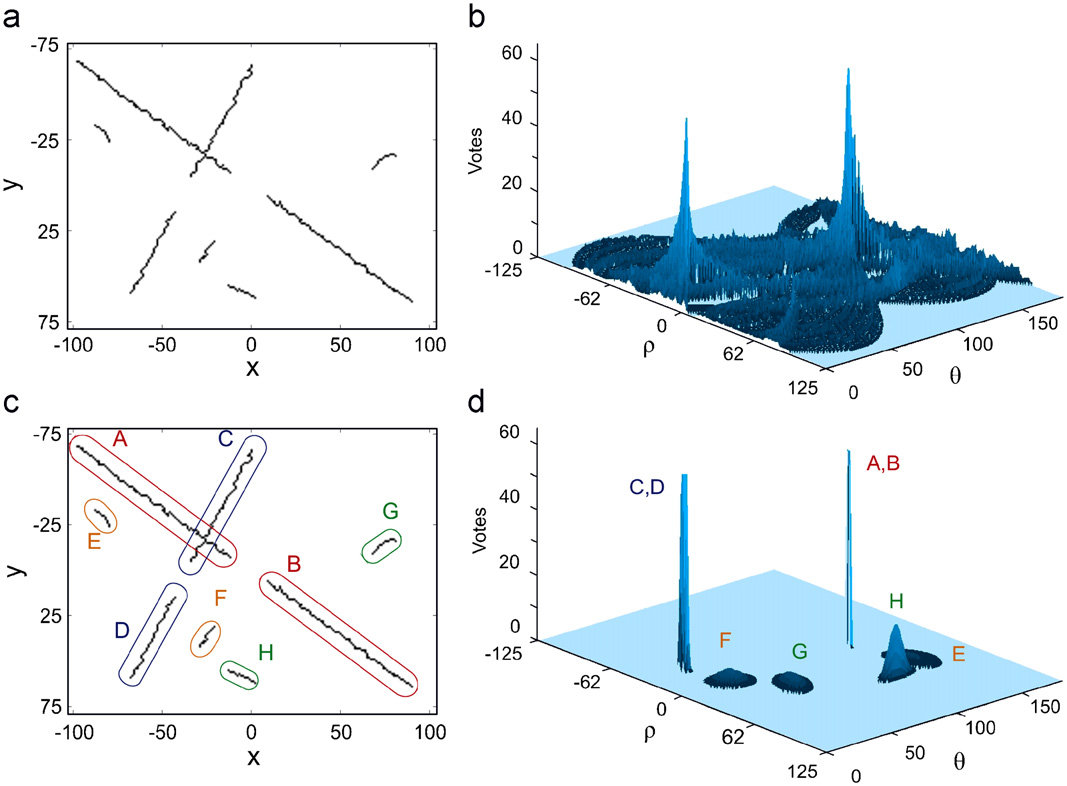
\includegraphics[width=0.5\columnwidth]{figures/hough_voting_demo.jpg}
\caption{Differences in the conventional versus Kernel-based Hough Transforms: (a) shows simple image with approximately straight line segments; (b) shows the voting map in the angle-radius space; (c) shows the clusters of pixels detected in KHT; (d) shows the voting map produced with the KHT technique, where the height of the A-B and C-D peaks have been truncated to improve the visualization. Reprinted from \cite{fernandes:2008}.}
\label{fig: hough demo}
\end{figure}
\begin{figure}
\centering
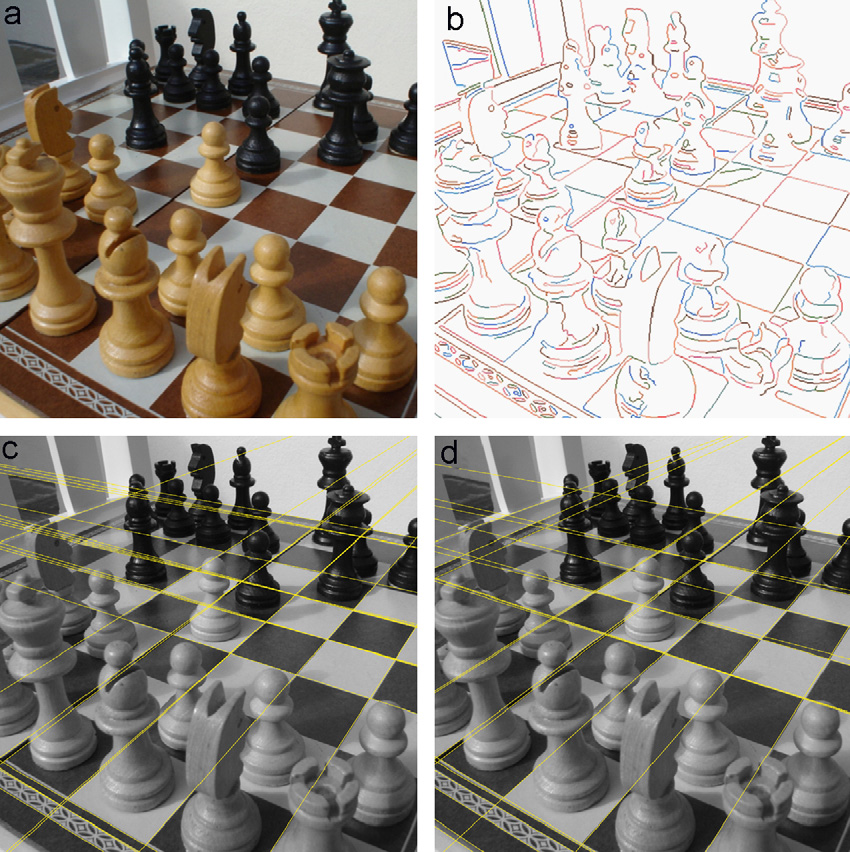
\includegraphics[width=0.5\columnwidth]{figures/hough_line_identification.jpg}
\caption{Line detection using the Kernel-based Hough Transform and conventional Hough Transform. (a) shows the input image; (b) shows the results of using a Canny edge detector; (c) shows the results produced by a conventional Hough Transform, with too-many lines detected in some places, while other lines are missed; (d) shows the results of the Kernel-based Hough Transform. Reprinted from \cite{fernandes:2008}}
\label{fig: hough results}
\end{figure}


Once streaks are identified, their approximate profile can be fit so that the portion of the image contaminated above a given level can be masked out. The brightness at which the wings of the streak are masked out must be balanced with the need to preserve as much of the image as possible.

The procedure used to identify streaks is described in Section~\ref{sec: algorithm}. The method to refine the fit to the identified streaks and to mask them out is described in Section~\ref{sec: line fitting}. The method's current implementation in the Rubin pipeline is described in Section~\ref{sec: implementation}.

\section{Method}
\subsection{The Streak Finding Algorithm}
\label{sec: algorithm}
In practice, some preprocessing of astronomical images helps KHT work smoothly: the map of ``detected'' pixels is used to produce a binary image, which removes background noise and significantly speeds up runtime by removing spurious clusters of points; then, a Canny filter is applied to detect the edges of objects in the image, which turns a streak into two approximately straight, parallel lines. At this point, KHT can be run on the processed image and will result in a small set of potential lines in the image. Figure~\ref{fig: algo steps} demonstrates these steps on a sample image.
\begin{figure}
\centering
\subfloat[]{{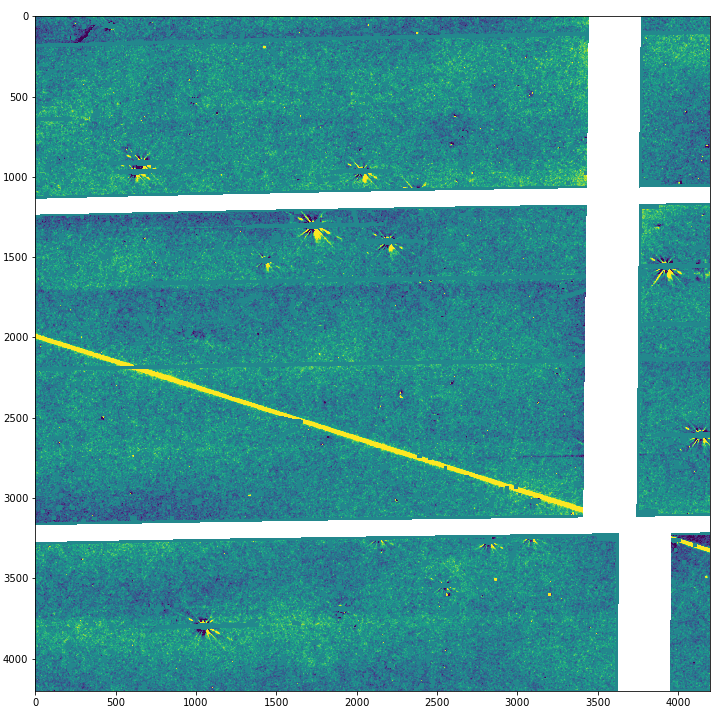
\includegraphics[width=0.32\columnwidth]{figures/HSC-R_visit23694_patch3,1_orig.png} }}
\qquad
\subfloat[]{{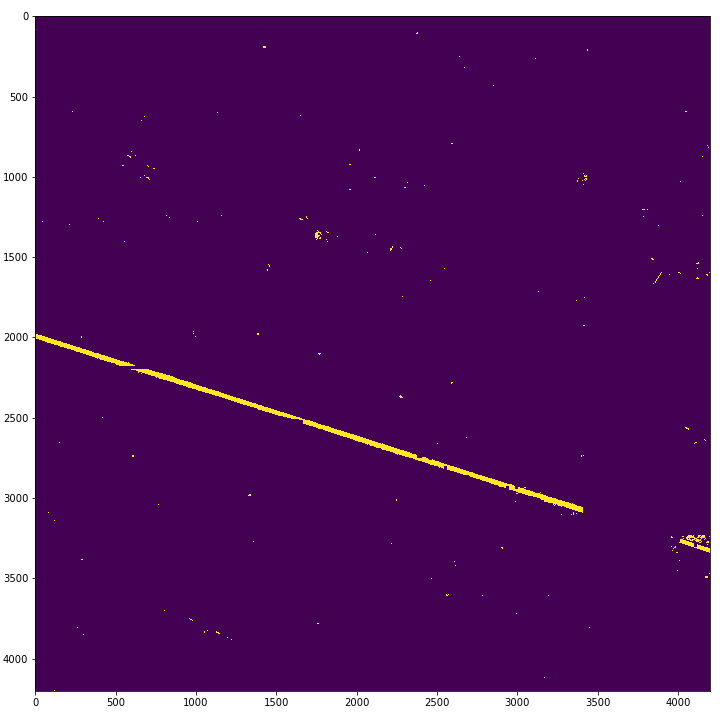
\includegraphics[width=0.32\columnwidth]{figures/HSC-R_visit23694_patch3,1_binary.png} }} \\
\subfloat[]{{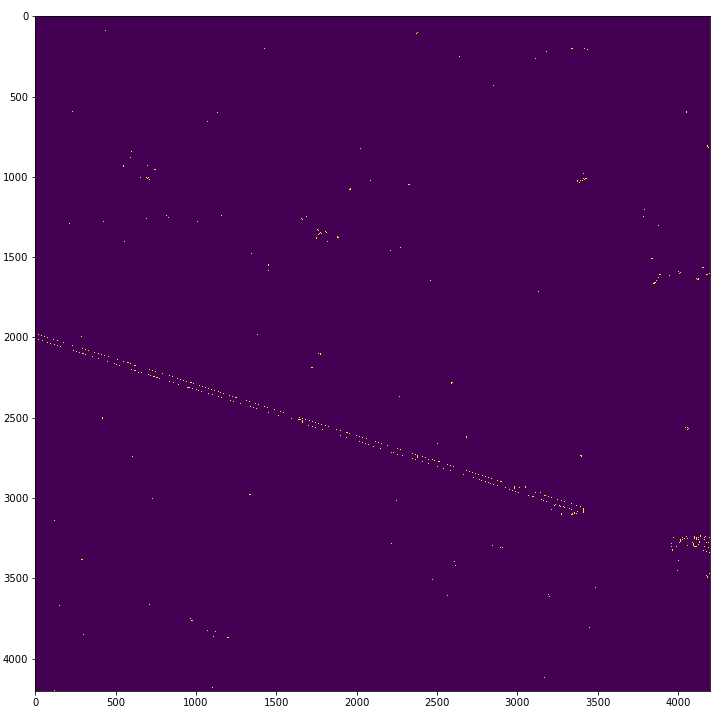
\includegraphics[width=0.32\columnwidth]{figures/HSC-R_visit23694_patch3,1_canny.png} }}
\qquad
\subfloat[]{{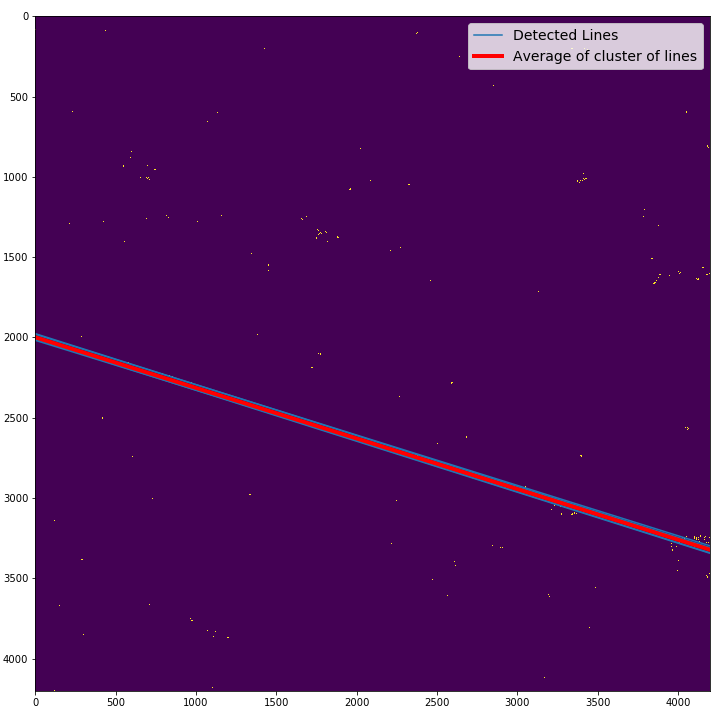
\includegraphics[width=0.32\columnwidth]{figures/HSC-R_visit23694_patch3,1_bestLines.png} }} \\
\subfloat[]{{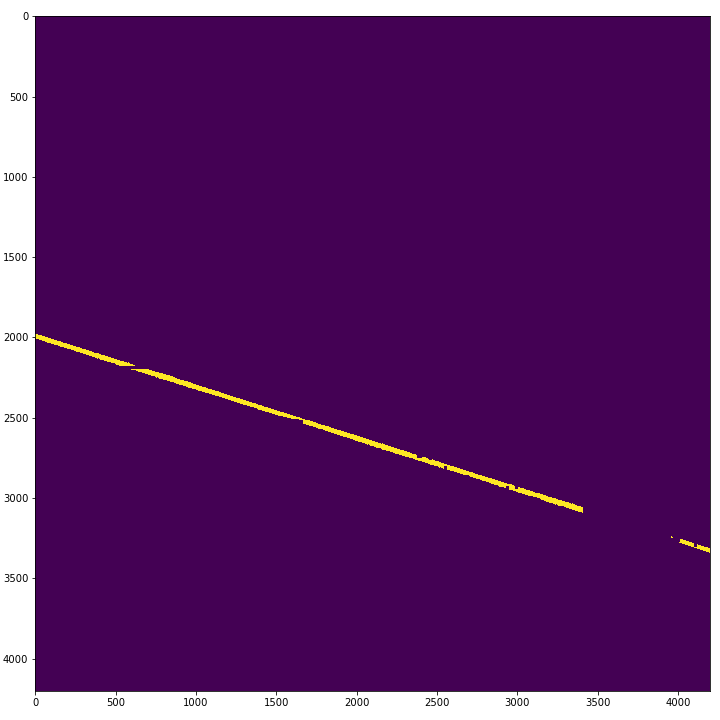
\includegraphics[width=0.32\columnwidth]{figures/HSC-R_visit23694_patch3,1_streakMask.png} }}
\qquad
\subfloat[]{{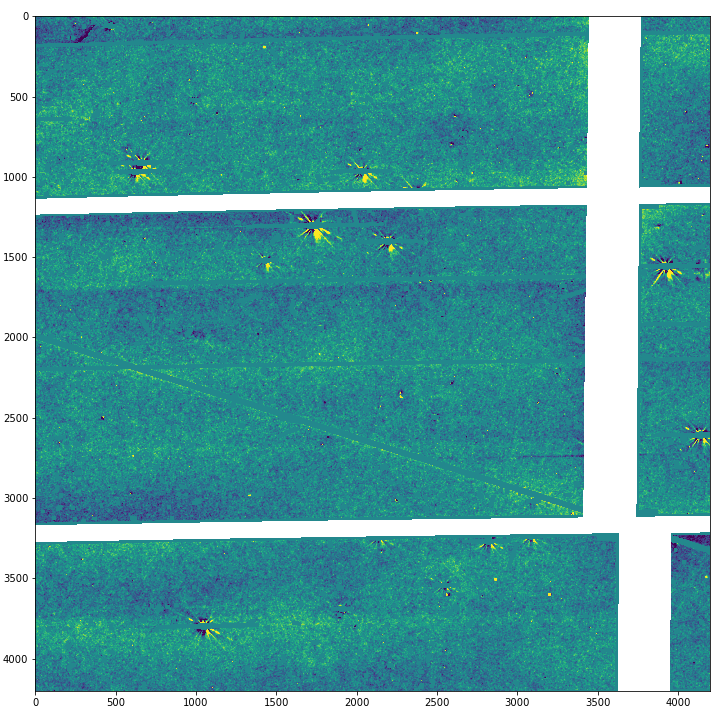
\includegraphics[width=0.32\columnwidth]{figures/HSC-R_visit23694_patch3,1_origMasked.png} }}  \\
\caption{Demonstration of the streak masking: (a) shows the original image, which is a warped difference image created from subtracting a clipped \texttt{deepCoadd} from a \texttt{deepCoadd\_directWarp}; (b) shows the mask of detected pixels in the image; (c) shows the result of using a Canny edge detector; (d) shows the lines detected by KHT in blue, with the line corresponding to the average position of the KHT lines is in red; (e) shows the mask fit to the detected streak; (f) shows the final image with the streak masked out.}
\label{fig: algo steps}
\end{figure}

KHT parameterizes lines with their angle and radius from the center of the image, and both KHT and the original Hough Transform discretize the angle-radius space in order to restrict possible lines to a finite number. Thus, further fitting is required to reconcile multiple lines fit to the same streak and to refine the exact position of the streak, for which the discretization may not be sufficiently accurate.


\subsection{Fitting the Streak Mask}
\label{sec: line fitting}

For a given streak in an image, KHT will typically result in a small set of likely lines, generally with at least one detection for each edge of the detected streak. From this set of likely lines, we want to produce a mask covering the portion of the image affected by the streak above a certain level. To do this, the results from KHT are first separated into clusters using the K-means clustering algorithm implemented in \texttt{sklearn.cluster.KMeans} (\citealt{Pedregosa:2011}). The best guess for the center of the streak is then estimated to be the average of the parameters for the likely lines in the cluster, shown in panel (d) of Figure~\ref{fig: algo steps}.

Given this best guess for the position of the streak, we then return to the original image to both refine the fit of the position and to fit its approximate profile. The streak is modeled as a line convolved along the perpendicular with a Moffat point spread function (PSF). The angle and radius of the line, plus the width of the Moffat profile, are all fit parameters, while the flux of the streak is determined by finding the best fit to the data given the other parameters of the model. The best fit of the model is determined by using the Newton-Raphson minimization method. Figure~\ref{fig: profile} shows the profile of a streak and the model fit to it. Given this model, the pixels above a given threshold in mJansky are used to make a mask.
\begin{figure}
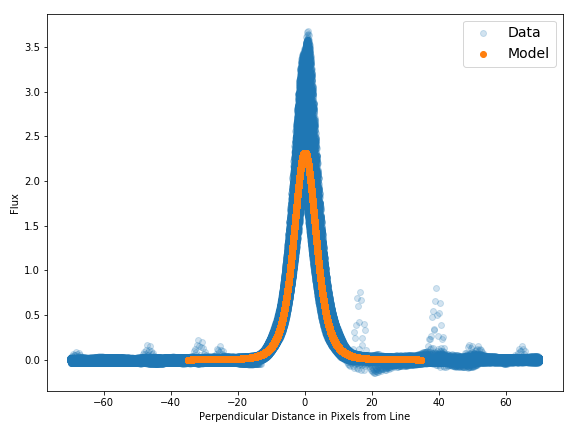
\includegraphics[width=\columnwidth]{figures//HSC-R_visit23694_patch3,1_StreakFit.png}
\caption{Image data at the location of a streak, with the model fit to the streak profile.}
\label{fig: profile}
\end{figure}

The final mask determined by this procedure is the intersection of the original map of ``detected'' pixels and the masks of any streaks detected in the image.


\section{Implementation in the DRP Pipeline}
\label{sec: implementation}

Streak masking is currently only attempted in the Data Release Production, where it is used in the construction of the coadded images. In \texttt{CompareWarpAssembleCoaddTask}, a naive model of the static sky is subtracted from each of the PSF-matched warps. Artifacts are then found by looking at detections in the difference image. Since the naive model of the sky is computed as a clipped mean, streaks, appearing in only one image, do not appear in it, and thus show up in the difference images. The algorithm \texttt{maskStreaks} is run on these warped difference images. For temporal artifact detection, apparent artifacts are filtered out if they appear in less than a certain fraction of difference images. However, artifacts that are determined to be streaks are filtered out without regard to how many images they appear in. This helps to ensure that streaks that overlap with other static objects, such as bright stars, are still removed. 

An example of the results of the image coaddition in the Gen3 pipeline with and without using streak masking is shown in Figure~\ref{fig: pipeline demo}.
\begin{figure}
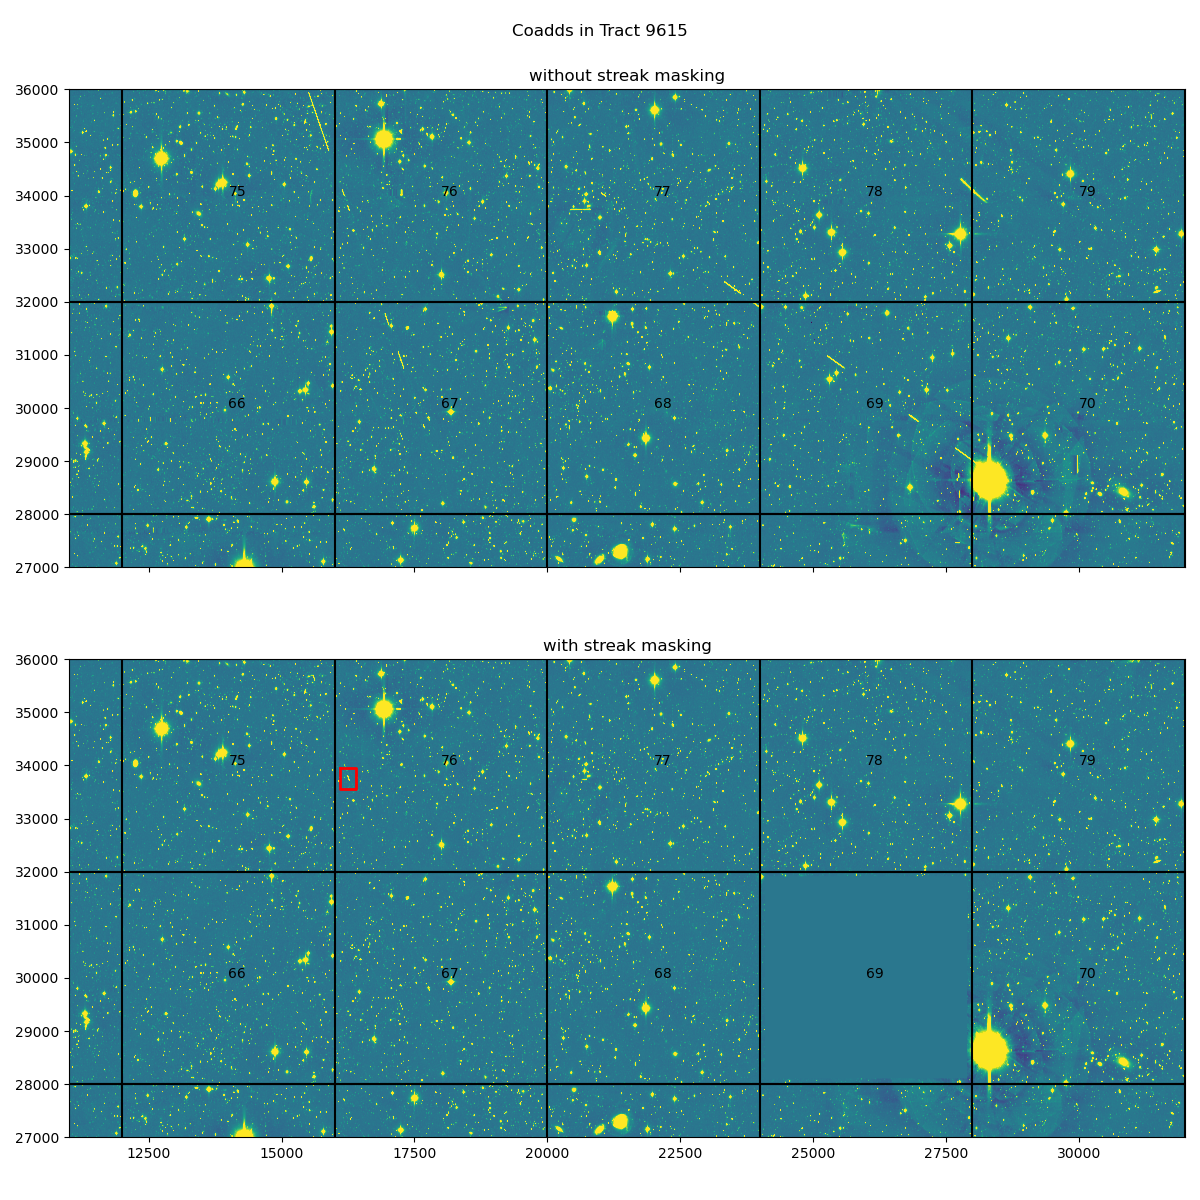
\includegraphics[width=\columnwidth]{figures/streakMasking_tractdemo_gen3.png}
\caption{The top panel shows a mosaic of several HSC-Y band coadds in Tract 9615, where patches $67$, $69$, $75$, $77$, $78$, and $79$ are affected by satellite trails, or possibly optical ghosts in the case of the streak on the border of patches $78$ and $79$. The lower panel shows the result of processing the data after streak masking was added to the pipeline. Patch $69$ is blank in the lower panel because processing failed at some point for that patch. The red box in the lower panel shows a small section of a streak that was not successfully masked.}
\label{fig: pipeline demo}
\end{figure}
A small portion of a streak appears to still be visible after the streak masking procedure. This may have been because the streak crossed the corner of the difference image, making it difficult to detect as a linear feature. Neighbouring images could be used to help detect streaks in this case, but that will be saved for future work.

Future work may also add this streak masking to the prompt processing pipeline for Rubin, but this has not yet been tested or implemented.

%\appendix
% Include all the relevant bib files.
% https://lsst-texmf.lsst.io/lsstdoc.html#bibliographies
\section{References} \label{sec:bib}
\renewcommand{\refname}{} % Suppress default Bibliography section
\bibliography{local}%,lsst,lsst-dm,refs_ads,refs,books}

% Make sure lsst-texmf/bin/generateAcronyms.py is in your path
\section{Acronyms} \label{sec:acronyms}
\addtocounter{table}{-1}
\begin{longtable}{p{0.145\textwidth}p{0.8\textwidth}}\hline
\textbf{Acronym} & \textbf{Description}  \\\hline

B & Byte (8 bit) \\\hline
DM & Data Management \\\hline
DMTN & DM Technical Note \\\hline
DRP & Data Release Production \\\hline
HSC & Hyper Suprime-Cam \\\hline
KHT & Kernel Hough Transform \\\hline
LSST & Legacy Survey of Space and Time (formerly Large Synoptic Survey Telescope) \\\hline
NCSA & National Center for Supercomputing Applications \\\hline
PSF & Point Spread Function \\\hline
\end{longtable}

% If you want glossary uncomment below -- comment out the two lines above
%\printglossaries





\end{document}
